\section{DCT wavelets}
L'obiettivo dell'analisi è la \textbf{riduzione delle ridondanze}, spostandosi in uno spazio dove le informazioni e i canali sono separati. 

Nel dominio diretto le componenti di un segnale $X$ sono tra loro significativamente correlate, quindi la stessa informazione è ridondante. Spostandosi nel dominio trasformato $Y = T[X]$, si cerca una rappresentazione dove le componenti siano molto meno correlate.

$Y$ può essere codificato in modo più efficiente di $X$, utilizzando solo le componenti del segnale che descrivono l'informazione. Lo spettro, per esempio, ha un contributo maggiore espresso con le basse frequenze al centro, quindi è possibile codificare solo una porzione determinata di energia.

In termini di compressione, sono necessari solo i bit delle componenti da tenere. Il modello di compressione permette di quantizzare con perdite trascurabili, in un cambio di spazio secondo due strategie:
\begin{itemize}
	\item Codificatore di \textbf{sorgente}, che riduce le ridondanze;
	\item Codificatore di \textbf{canale}, che incrementa l'immunità al rumore.
\end{itemize}

\subsection{Codifica con trasformate}
Questo algoritmo introduce perdita ed è computazionalmente costoso, a causa del calcolo delle trasformate. Una trasformata lineare e reversibile è usata per il mapping dell'immagine in un set di coefficienti che vengono poi quantificati e codificati.

Il mapping può essere effettuato secondo diverse metodologie, a seconda della capacità di decorrelazione dei dati, semplicità di realizzazione e altri fattori.

La KLT (analisi alle componenti principali) è la trasformata ottima, ma è computazionalmente inefficiente. DCT, invece, approssima il comportamento ottimo, ed è usata negli algoritmi di codifica più utilizzati (jpeg, mpeg).

La trasformata wavelet permette la \textbf{multirisoluzione} (JPEG-2000), e funziona secondo il principio di determinazione di Heisenberg, trovando un compromesso tra le frequenze e il dominio temporale lavorando con tradeoff.

Data una funzione $f(x)$, la sua DFT $F(u)$ è:
$$F(u) = \frac{1}{M} \sum_{x=0}^{M- 1}f(x)e^{-j\frac{2\pi}{M}ux} = \frac{1}{M} \sum_{x=0}^{M- 1}f(x)g(u, x)$$
$$g(u, x) = e^{-j\frac{2\pi}{M}ux}$$

La trasformata è lineare e invertibile, e $g(u, x)$ è detto \textbf{kernel} della trasformazione diretta, da cui dipendono le proprietà. I kernel devono essere \textit{invertibili}, \textit{lineari} e \textit{separabili}.

Trasformata di Fourier discreta 1D:
$$e^{-j\frac{2\pi}{M}ux} = \cos\big(\frac{2\pi}{M}ux\big) + j\sin\big(\frac{2\pi}{M}ux\big)$$

\begin{figure}[h]
	\centering
	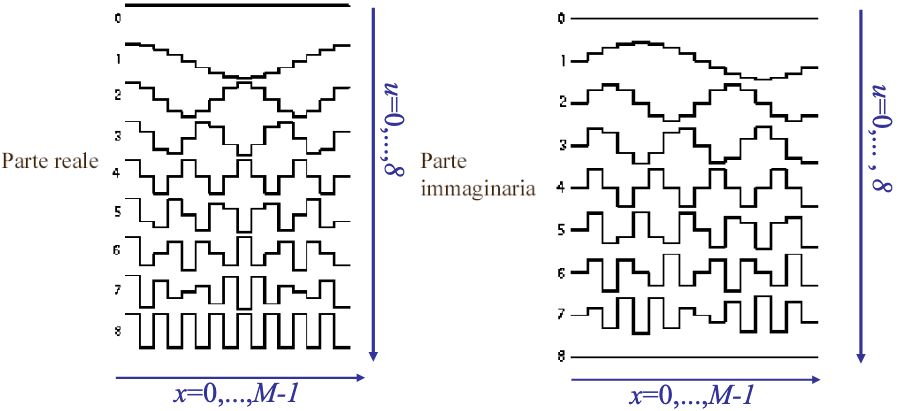
\includegraphics[scale=0.48]{Lezioni/Immagini/ondequadrate}
\end{figure}

Il segnale di partenza è proiettato in base al suo tempo e spazio con le sue parti reale e immaginaria. Seno e coseno hanno simmetria rispettivamente dispari e pari, e trasformando si osserva l'influenza di ciascuna componente. 

La trasformata coseno discreta (DCT) è lineare, con kernel diretto uguale a quello inverso (simmetria speculare), separabile e simmetrico. La componente continua è legata al \textbf{valore medio} dell'immagine (0, 0). 
$$T(u) = \sum_{x=0}^{M- 1}f(x)g(u, x) \qquad g(x, u) = \alpha(u) \cos\Big[\frac{(2x + 1)\pi u}{2N}\Big]$$

$$\alpha(u) = \begin{cases}
\sqrt{\frac{1}{N}} & u = 0 \\
\sqrt{\frac{2}{N}} & u = 1, 2, \dots, N - 1^{}
\end{cases}$$

La separabilità permette di calcolare la trasformata 2D tramite applicazioni successive della trasformata 1D alle righe e alle colonne, senza perdita di informazione. Ciascun blocco è costituito da $N \times N$ sottoblocchi.

Una maggiore quantità di informazione è presente nei primi coefficienti della DCT, rispetto allo stesso numero di coefficienti della DFT.

\begin{figure}[h]
	\centering
	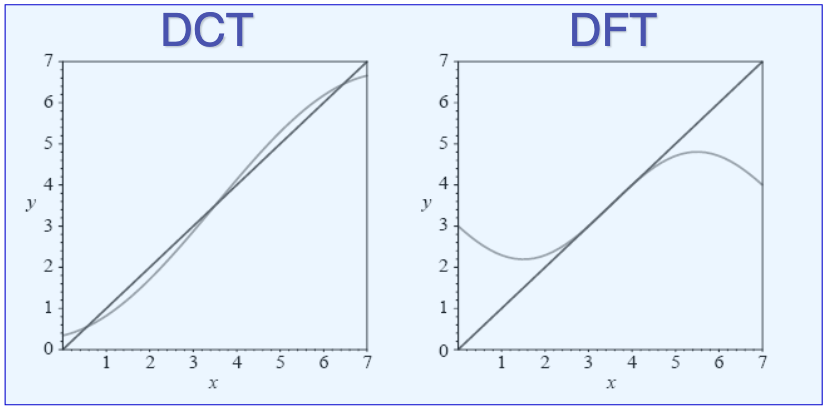
\includegraphics[scale=0.27]{Lezioni/Immagini/dctdft}
\end{figure}

\subsection{Analisi multirisoluzione}
Le immagini sono generalmente costituite da regioni connesse che formano gli oggetti, omogenee rispetto a una qualche proprietà.

L'analisi multirisoluzione permette di mettere in evidenza sia le immagini a bassa frequenza che quelle ad alta, con segnali e campioni di dimensioni diverse, concentrandosi su differenti posizioni nello spettro. 

Le caratteristiche locali di un'immagine sono contraddistinte da variazioni statistiche locali, dovute a discontinuità fra regioni omogenee. Caratteristiche nascoste a una data risoluzione possono essere individuabili a un'altra.

La tecnica più frequente è l'\textbf{analisi piramidale}, che parte dalla risoluzione massima e progressivamente sottocampiona, evidenziando i cambiamenti tra i dettagli e le perdite tra un livello e l'altro ricostruendo ogni volta l'immagine con meno dettagli. I pixel mancanti vengono approssimati tramite wavelet.

Il segnale è decomposto in un insieme di sottosegnali (sottobanda, analisi), passando attraverso filtri complementari, ciascuno dei quali agisce su una fascia di frequenze. Ricampionando, filtrando e ricombinando le sottobande (sintesi) si ottiene un'approssimazione $\hat{x}(n)$ dell'originale, non incorrendo in aliasing. 

Ciascuna sottobanda $(y_0(n), y_1(n))$ è ottenuta filtrando con un passa-banda $(h_0(n), h_1(n))$ il segnale originale. Poiché la sottobanda ha spettro limitato e pari a metà dell'originale, è possibile sottocampionare senza perdita di informazione. 

\begin{figure}[h]
	\centering
	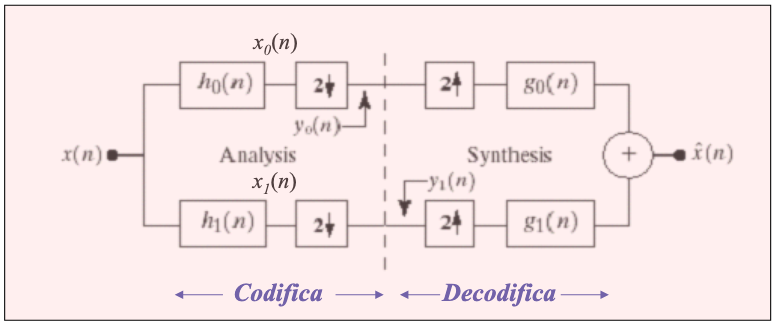
\includegraphics[scale=0.3]{Lezioni/Immagini/sottobande}
\end{figure}

Imponendo $\hat{x}(n) = x(n)$, si trovano le opportune coppie di filtri di sintesi e corrispondenti filtri di analisi che garantiscono una perfetta ricostruzione. In caso di più dimensioni (separabili), possono esserci $n$ filtri per righe e colonne che mettono in evidenza diverse porzioni di frequenze rispetto alla direzione. Flitraggio e sottocampionamento avvengono quindi in due fasi successive.

Si ottengono 4 immagini di output: $dV(m, n)$, $dH(m, n)$, $dD(m, n)$ le immagini nelle 3 dimensioni per le alte frequenze, e $a(m, n)$ l'immagine approssimata. Ciascuna sottobanda a sua volta può essere scomposta in 4 ulteriori sottobande.

\begin{figure}[h]
	\centering
	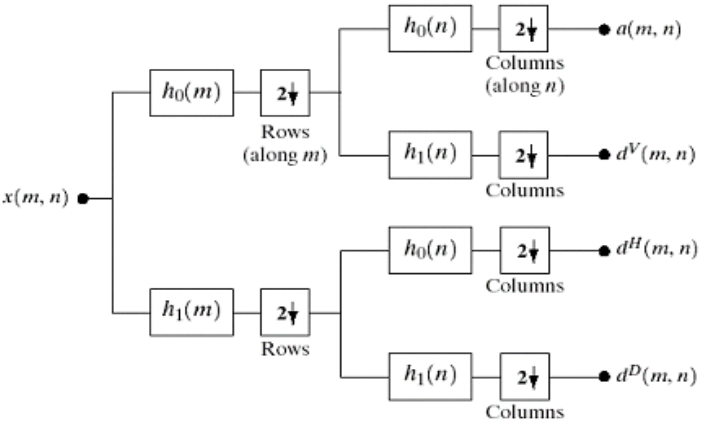
\includegraphics[scale=0.5]{Lezioni/Immagini/sottobande2d}
\end{figure}

Visivamente, è immediata la correlazione fra filtri di analisi e sintesi corrispondenti: sono ortonormali, cioè ortogonali a norma unitaria, e permettono una ricostruzione error-free in ciascun livello che a sua volta viene approssimato.

Dato che le statistiche locali sono facilmente modellabili e presentano molti valori nulli, questa codifica è particolarmente vantaggiosa per la compressione: non tutto l'istogramma viene occupato, oppure ci sono poche alte frequenze che possono essere eliminate. L'approccio di denoising per ridurre il rumore è utilizzato nelle applicazioni mediche.

Nell'analisi multirisoluzione, il filtro passa-basso è una \textit{funzione di scala} (MRA), mentre il passa-alto è una \textit{wavelet} generata a partire da una wavelet madre. Ogni approssimazione differisce dalla più vicina di un fattore 2.

Le wavelet descrivono la differenza di informazione fra due approssimazioni adiacenti. La formula in notazione monodimensionale è:
$$f(x)  = \frac{1}{\sqrt{M}} \sum_{k} W_\varphi (j_0, k) \varphi_{j_0, k} (x) + \frac{1}{\sqrt{M}} \sum_{j=j_0}^{J}\sum_{k} W_\psi(j, k)\psi_{j, k}(x)$$
$\varphi(x)$ è la funzione di scaling, con i relativi coefficienti di approssimazione. $\psi(x)$ è la wavelet madre, con i relativi coefficienti di dettaglio.

Tramite imposizione di equivalenze tra prodotti, è possibile misurare le variazioni lungo le righe, le colonne e le diagonali. 

Trasformando con la wavelet, è possibile pesare ogni contributo per capire quali frequenze e bande hanno influenza maggiore, valutando le features che caratterizzano l'immagine. 

Per calcolare gli edge, si ha il segnale di partenza in una somma di contributi: la parte interessata (per esempio il filtro passa alto $\psi$) viene tenuta applicando la formula, mentre le altre componenti con frequenze basse vengono annullate. 

Annullando anche i termini di edge orizzontali a tutte le scale e ricostruendo (sintesi) a partire da questi dati, si isolano i soli edge verticali.

Un altro approccio è il denoising, a partire dalle wavelet. La ricostruzione è effettuata dopo aver posto una soglia alta sui coefficienti a tutte le risoluzioni, accettando solo i valori al di sopra. 

 \begin{wrapfigure}{L}{0.55\textwidth}
	\vspace{-5pt}
	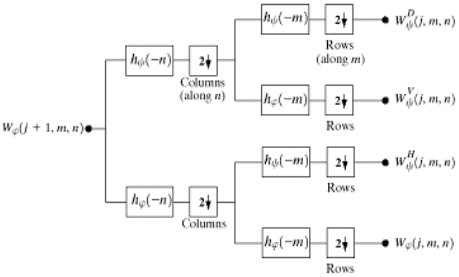
\includegraphics[width=0.55\textwidth]{Lezioni/Immagini/wct2}
	\vspace{-50pt}
\end{wrapfigure}

L'immagine originale è una risonanza magnetica con un rumore bianco additivo o moltiplicativo, a cui viene applicata la procedura di denoising:
\begin{enumerate}
	\item Scelta della funzione wavelet;
	\item Scelta del numero di livelli;
	\item Sogliatura dei coefficienti di wavelet ed eliminazione di quelli inferiori;
	\item Ricostruzione a partire dall'immagine approssimata all'ultima scala.
\end{enumerate}

Riducendo il rumore, si ha notevole perdita di dettaglio anche sugli edge, applicando soglie a tutte le risoluzioni. Agendo solo sulla risoluzione massima, si ha una perdita minore.

Per il principio di indeterminazione di Heisenberg, la distanza per ogni punto esatto di una funzione è infinitesima: pertanto, la risoluzione nelle frequenze è indefinita. Nel dominio trasformato, è nota l'informazione per ogni valore di $f$, ma $\delta x$ è infinito. 

In altre parole, in base al dominio, una dimensione è indeterminata. Il prodotto delle due, che corrisponde all'area, è sempre maggiore di un valore $K$:
$$\delta t \times \delta v \geq K$$
Nelle wavelet, è possibile determinare precedentemente una delle due dimensioni, avendo contemporaneamente informazione spaziale e frequenziale.

